\chapter{الخلط والذوبان}\label{ch:g2:mixing-and-dissolving}

يسقط مكعب سكر في فنجان شاي ساخن. تحرّكه ملعقة، فيتفتت المكعب، وبعد
لحظة لا يبقى شيء يُرى: يبدو الشاي تمامًا كما كان من قبل. ومع ذلك صار
طعم الشاي حلوًا. لم يختفِ السكر --- إنه مختبئ في الشاي. يتحدث هذا الفصل
عن جمع الأشياء معًا، وعن الأشياء التي تبدو كأنها تختفي حين نفعل ذلك.

\begin{omfigure}
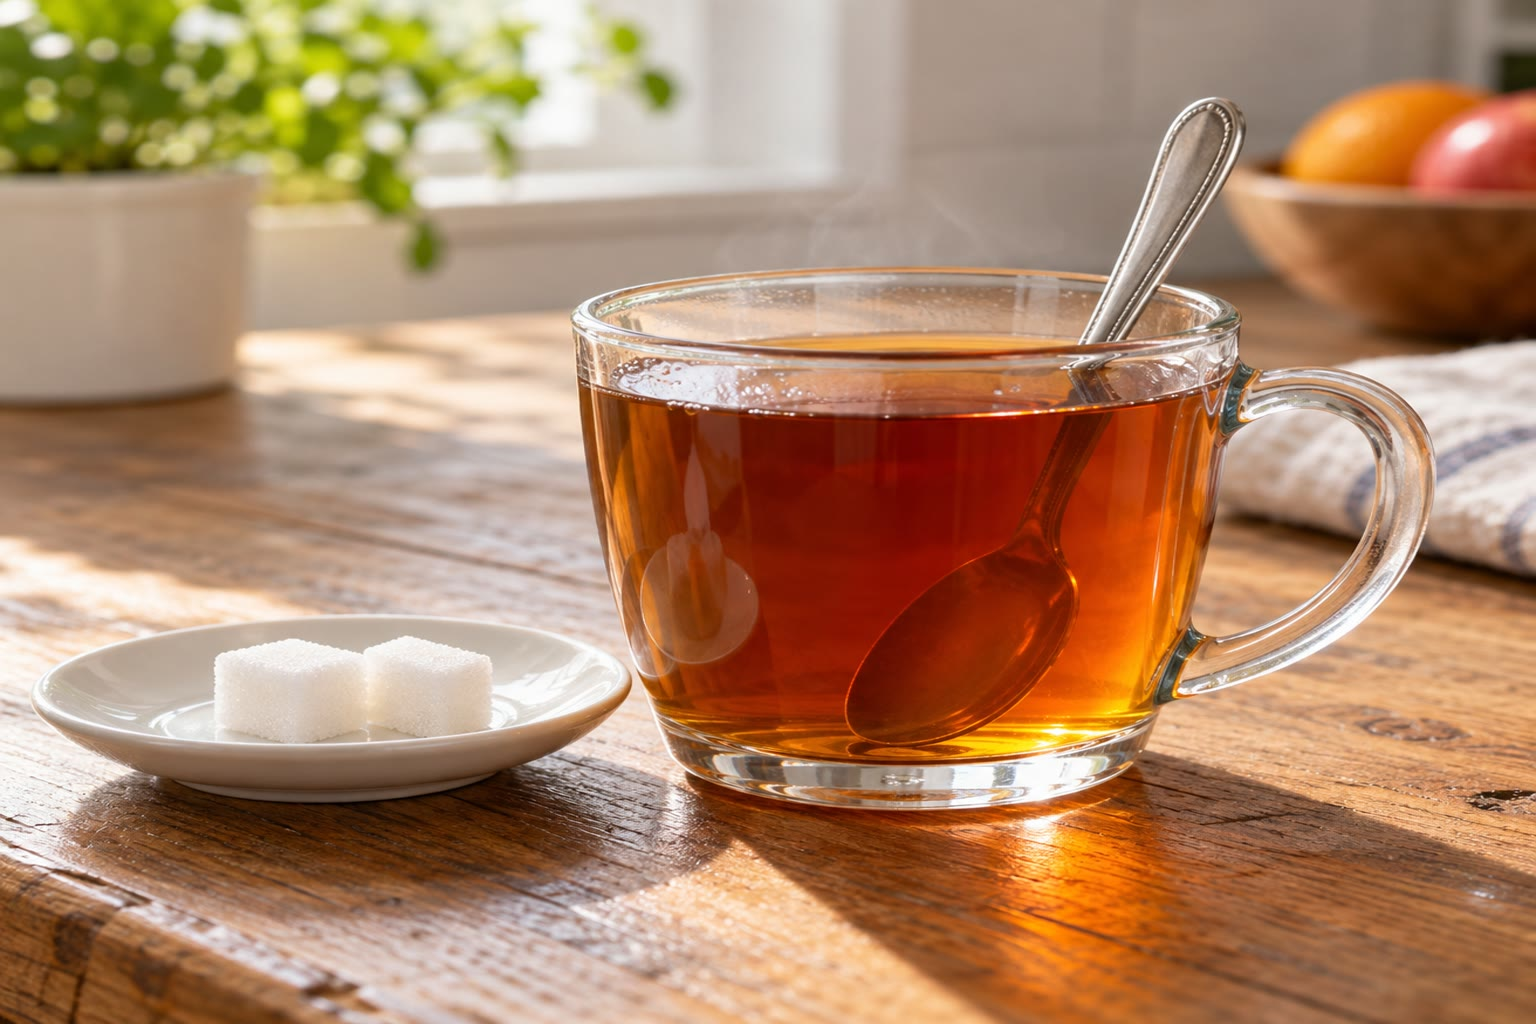
\includegraphics[width=0.55\linewidth]{images/book1/ai/g2-tea-sugar.jpg}

{\small فنجان شاي ومكعبا سكر. إذا حُرّك السكر في الشاي اختفى عن العين،
لكنه لم يختفِ عن الذوق.}
\end{omfigure}

\section{خلط الأشياء معًا}

\begin{definition}[الخلط]\label{def:g2:mixing-and-dissolving:mix}
\emph{الخلط}\index{خلط} أن نضع أشياء مختلفة معًا، وكثيرًا ما نحرّكها.
وما نحصل عليه خليط من هذه الأشياء.
\end{definition}

\begin{example}[صحن من الموسلي]\label{ex:g2:mixing-and-dissolving:muesli}
نصبّ الشوفان والزبيب والجوز والبذور في صحن واحد: هذا خليط. وإذا
دققت النظر رأيت كل مكوّن، واستطعت أن تلتقطه من جديد بأصابعك ---
فالزبيبة تبقى زبيبة، والجوزة تبقى جوزة.
\end{example}

\begin{example}[الشراب في الماء]\label{ex:g2:mixing-and-dissolving:syrup}
يمكن أيضًا \omterm{def:g2:mixing-and-dissolving:mix}{خلط} سائلين. إذا صببنا شرابًا أحمر في كأس ماء نزل إلى
الأسفل في دوامات ملونة؛ وبعد التحريك تصير الكأس كلها وردية بالتساوي.
ولا تستطيع العين بعد ذلك أن تميّز الشراب من الماء.
\end{example}

\begin{omfigure}
\begin{minipage}[t]{0.48\linewidth}\centering
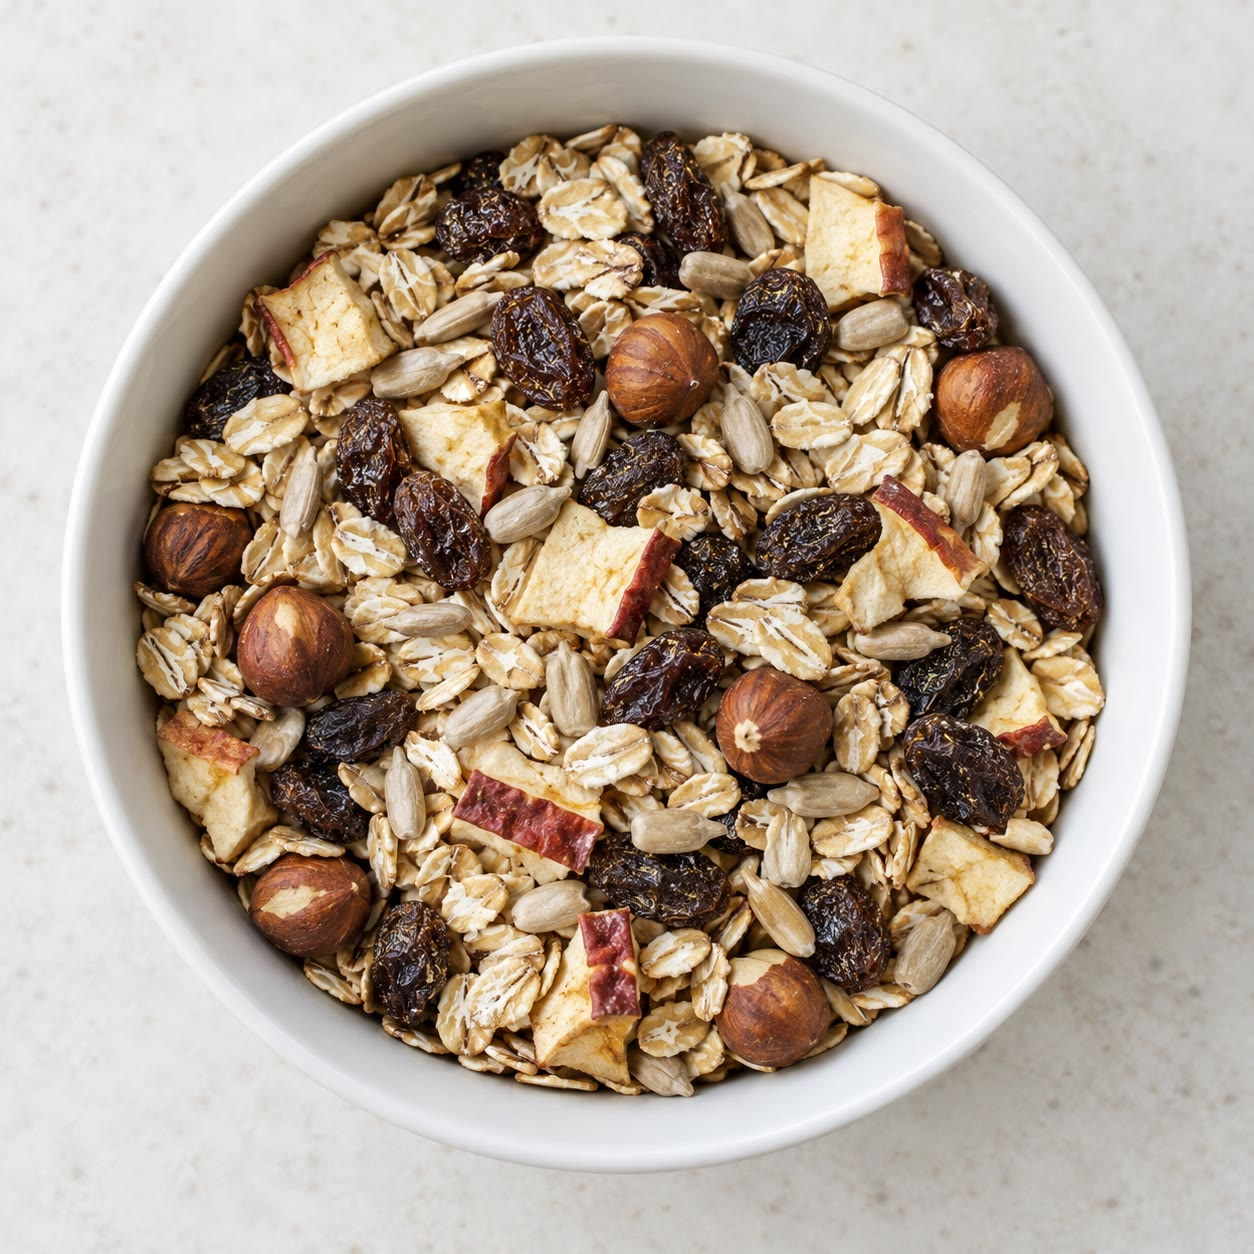
\includegraphics[width=\linewidth,height=4.6cm,keepaspectratio]{images/book1/ai/g2-muesli.jpg}

{\small الموسلي: خليط لا يزال كل جزء منه يُرى.}
\end{minipage}\hfill
\begin{minipage}[t]{0.48\linewidth}\centering
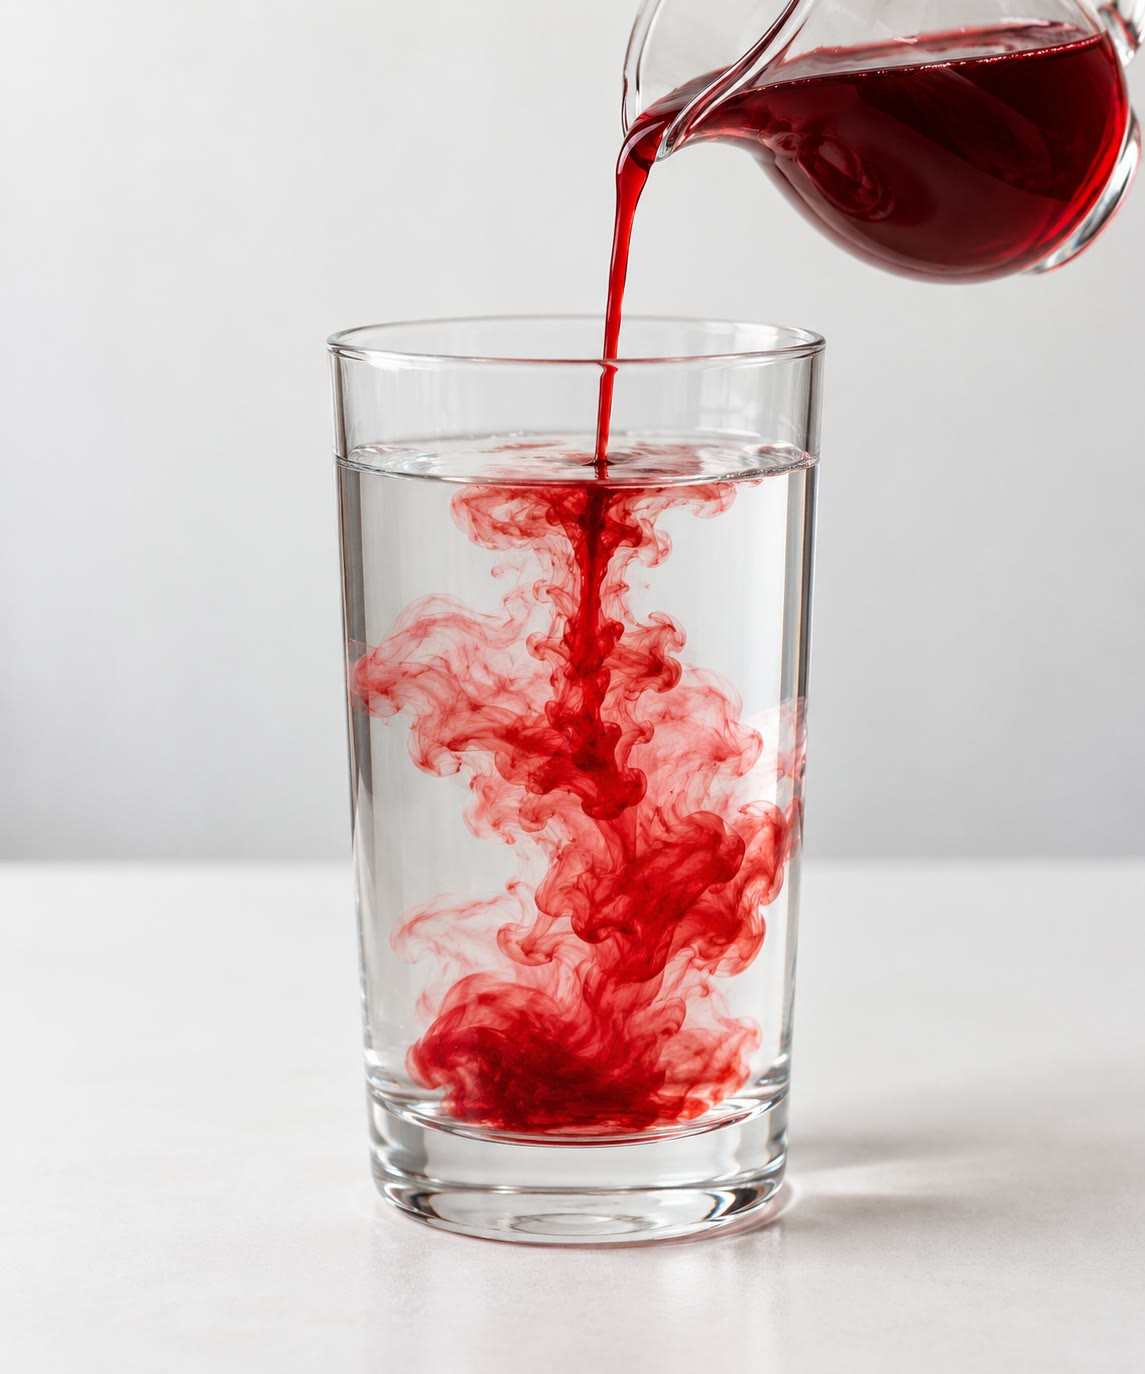
\includegraphics[width=\linewidth,height=4.6cm,keepaspectratio]{images/book1/ai/g2-syrup-in-water.jpg}

{\small شراب يُصبّ في الماء: سائلان يختلطان.}
\end{minipage}
\end{omfigure}

\begin{remark}[الخلط لا يُتلف شيئًا]\label{rem:g2:mixing-and-dissolving:nothing-lost}
حين نخلط الأشياء لا يضيع شيء ولا يُصنع شيء جديد. فالشوفان والزبيب
والجوز كلها لا تزال في الصحن. وسيبيّن فصل لاحق كيف نفصل الخليط من
جديد.
\end{remark}

\section{أشياء تذوب}

\begin{definition}[الذوبان والمحلول]\label{def:g2:mixing-and-dissolving:dissolve}
نقول إن جسمًا صلبًا \emph{يذوب}\index{ذوبان} في الماء إذا خلطناه بالماء
وحرّكناه فاختفى عن العين وترك السائل \emph{رائقًا}، أي نرى من خلاله.
السكر والملح يذوبان في الماء. والسائل الرائق الذي نحصل عليه يسمى
\emph{محلولًا}\index{محلول}: الماء المحلّى محلول سكر، والماء المالح
محلول ملح.
\end{definition}

\begin{example}[مكعب سكر في كأس ماء]\label{ex:g2:mixing-and-dissolving:cube}
نضع مكعب سكر في قاع كأس ماء ساكن. فتلين زواياه ويصغر، وتصعد منه
خيوط متموجة عبر الماء. إذا حرّكنا اختفى في أقل من دقيقة. وإذا لم
نحرّك اختفى أيضًا، لكن ببطء أكبر بكثير.
\end{example}

\begin{remark}[الرائق ليس هو عديم اللون]\label{rem:g2:mixing-and-dissolving:clear}
الشاي بني وماء الشراب وردي، لكننا نرى من خلال كليهما: فهما رائقان.
يمكن أن يكون \omterm{def:g2:mixing-and-dissolving:dissolve}{للمحلول} لون. أما ما لا يكون في \omterm{def:g2:mixing-and-dissolving:dissolve}{المحلول} أبدًا فقطع تطفو
فيه أو طبقة في قاعه.
\end{remark}

\begin{method}[هل يذوب؟]\label{met:g2:mixing-and-dissolving:test}
لتعرف هل \omterm{def:g2:mixing-and-dissolving:dissolve}{يذوب} جسم صلب في الماء:
\begin{enumerate}
  \item ضع قليلًا منه في كأس ماء؛
  \item حرّك، ثم انتظر بضع دقائق؛
  \item انظر من خلال الكأس:
    \begin{itemize}
      \item رائق، ولا شيء في القاع: الجسم الصلب قد ذاب؛
      \item عكر، أو طبقة في القاع: الجسم الصلب لم يذب.
    \end{itemize}
\end{enumerate}
\end{method}

\section{أشياء لا تذوب}

\begin{proposition}[الرمل والطباشير لا يذوبان]\label{prop:g2:mixing-and-dissolving:not}
كثير من الأجسام الصلبة لا \omterm{def:g2:mixing-and-dissolving:dissolve}{يذوب} في الماء: الرمل، والطباشير، والتراب،
والحصى، والدقيق. إذا حرّكناها في الماء جعلته عكرًا؛ وإذا تُركت ساكنة
نزلت واستقرت في القاع، وعاد الماء فوقها أصفى. ومهما طال التحريك فإنها
لا تختفي أبدًا.
\end{proposition}

\begin{example}[مرطبان من الماء الموحل]\label{ex:g2:mixing-and-dissolving:mud}
إذا رججنا تراب الحديقة في مرطبان ماء صار الماء بنيًا عكرًا. وبعد ساعة
يستقر التراب والحصى الصغير في طبقة داكنة في القاع، وتطفو في الأعلى
بضع أوراق ميتة، ويبقى الماء بينهما عكرًا قليلًا. لم يذب التراب.
\end{example}

\begin{omfigure}
\begin{minipage}[t]{0.48\linewidth}\centering
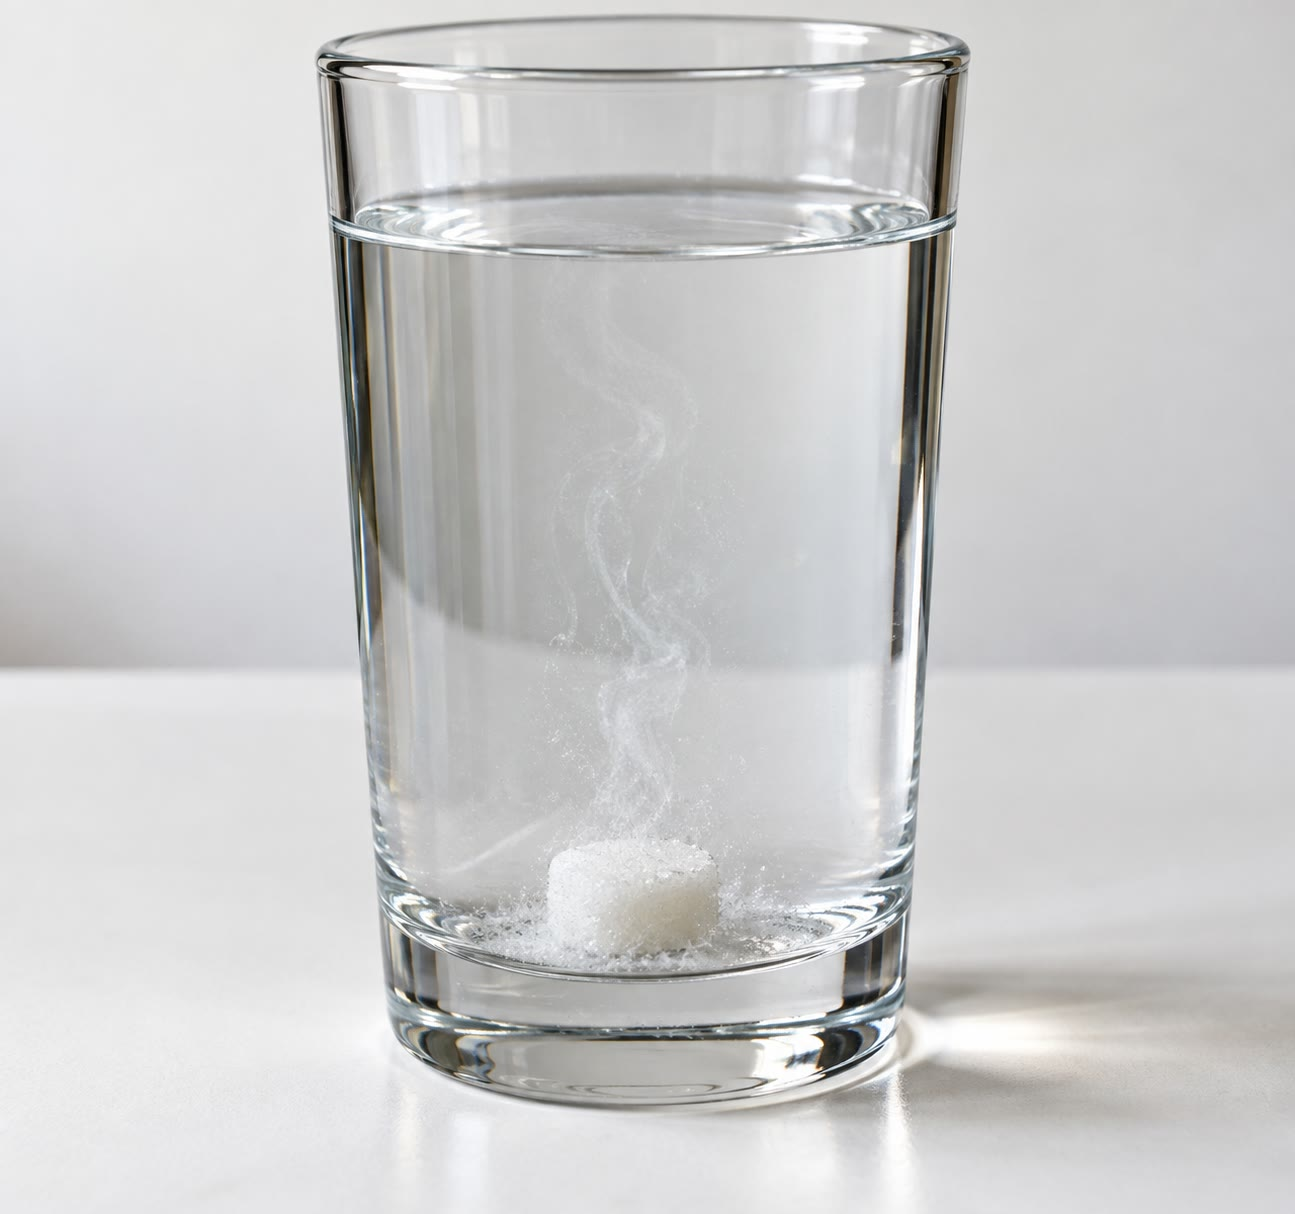
\includegraphics[width=\linewidth,height=4.6cm,keepaspectratio]{images/book1/ai/g2-sugar-cube-dissolving.jpg}

{\small السكر \omterm{def:g2:mixing-and-dissolving:dissolve}{يذوب}: خيوط تصعد من المكعب.}
\end{minipage}\hfill
\begin{minipage}[t]{0.48\linewidth}\centering
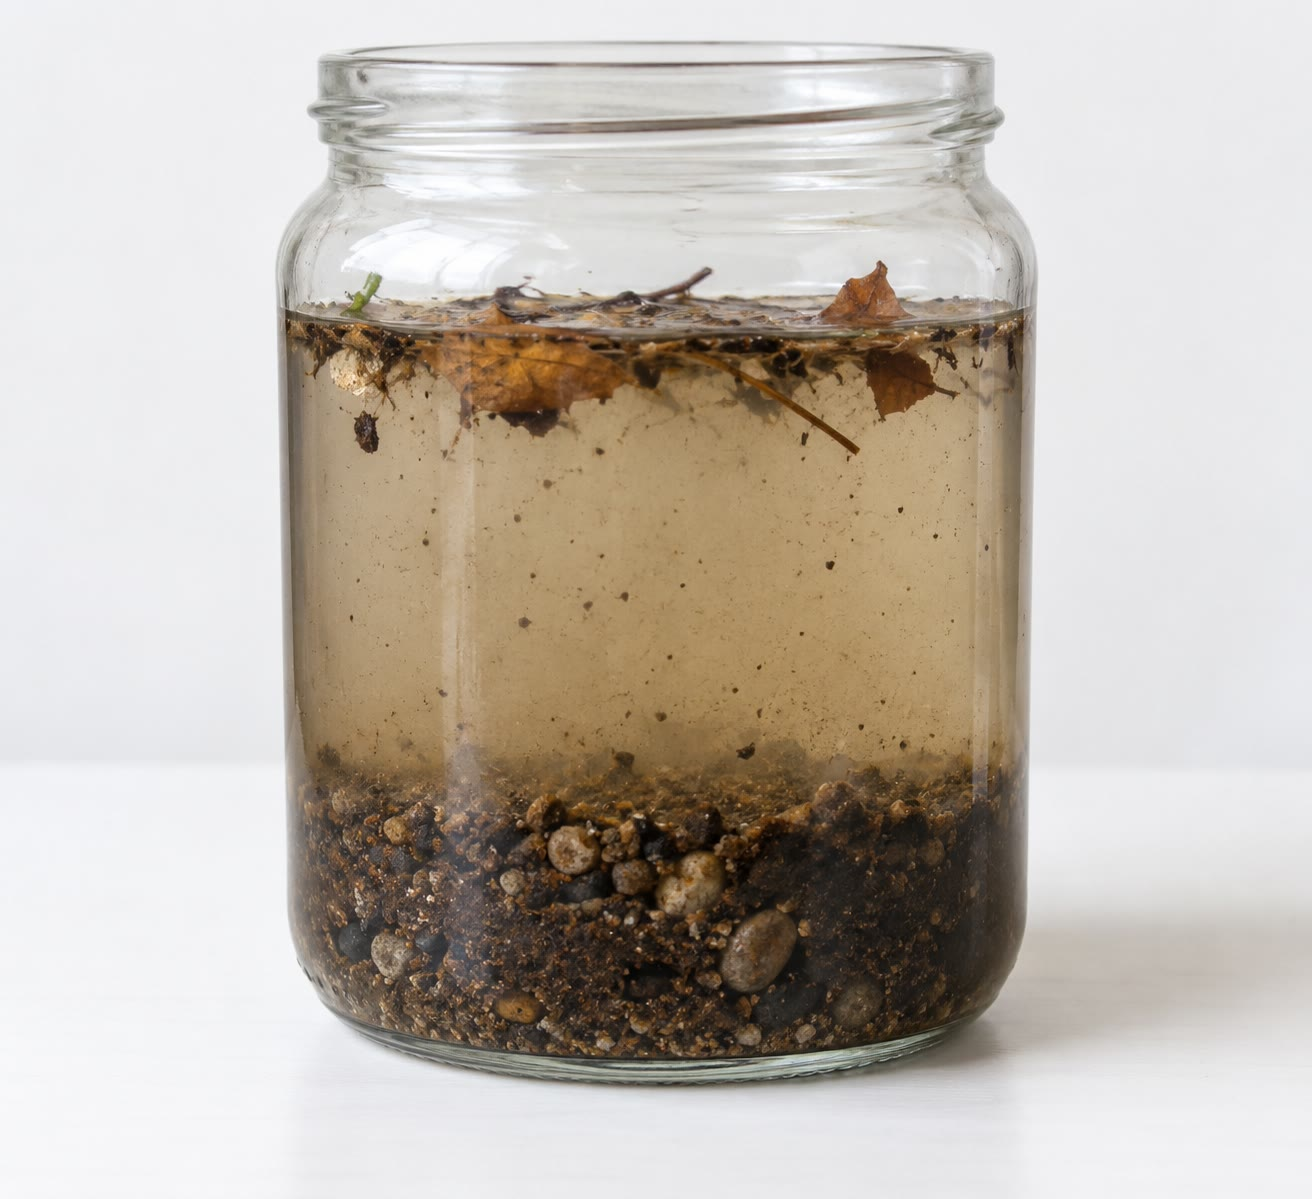
\includegraphics[width=\linewidth,height=4.6cm,keepaspectratio]{images/book1/ai/g2-muddy-jar.jpg}

{\small التراب لا \omterm{def:g2:mixing-and-dissolving:dissolve}{يذوب}: يستقر في القاع.}
\end{minipage}
\end{omfigure}

\begin{omfigure}
\begin{tikzpicture}[font=\small, scale=1.35]
  \pic[transform shape] at (0,0) {beaker={0.7}{omWater!70}};
  \fill[brown!55] (4.2,0) rectangle (5.8,0.22);
  \pic[transform shape] at (5,0) {beaker={0.7}{brown!12}};
  \fill[brown!55] (4.2,0) rectangle (5.8,0.22);
  \draw[omGlass, line width=0.7pt] (4.2,0.22) -- (4.2,0) -- (5.8,0) -- (5.8,0.22);
  \foreach \x/\y in {4.4/0.32,4.75/0.45,5.1/0.3,5.5/0.5,4.6/0.7,5.3/0.8,4.9/1.0}
    \fill[brown!60] (\x,\y) circle (0.025);
  \node[align=center, anchor=north] at (0,-0.15)
    {\textbf{السكر} في الماء بعد التحريك:\\ رائق، ولا شيء في القاع};
  \node[align=center, anchor=north] at (5,-0.15)
    {\textbf{الرمل} في الماء بعد التحريك:\\ عكر، وطبقة في القاع};
  \draw[<-, omProp, thick] (6.0,0.11) -- (7.0,0.11)
    node[right, text=black] {الرمل};
\end{tikzpicture}

{\small اختبار \cref{met:g2:mixing-and-dissolving:test}: السكر
\omterm{def:g2:mixing-and-dissolving:dissolve}{يذوب}، والرمل لا \omterm{def:g2:mixing-and-dissolving:dissolve}{يذوب}.}
\end{omfigure}

\section{ما يذوب يبقى موجودًا}

\begin{proposition}[الجسم الصلب الذائب لا يزال في الماء]\label{prop:g2:mixing-and-dissolving:still-there}
حين \omterm{def:g2:mixing-and-dissolving:dissolve}{يذوب} جسم صلب فإنه لا يتلاشى: بل ينتشر في الماء كله، في قطع أصغر
بكثير من أن تُرى. وتدل علامتان على أنه لا يزال موجودًا:
\begin{itemize}
  \item الشاي المحلّى طعمه حلو، وماء البحر طعمه مالح؛
  \item حين يجف الماء يبقى الجسم الصلب بعده.
\end{itemize}
\end{proposition}

\begin{remark}[لا تذوّق في المختبر]\label{rem:g2:mixing-and-dissolving:no-tasting}
نعرف أن الشاي حلو لأن الشاي طعام. أما في المختبر فلا أحد يتذوق أي
شيء أبدًا، ولا حتى سائلًا يشبه الماء: فالعلامة الثانية، أي ترك الماء
يجف، هي التي يستعملها الكيميائيون.
\end{remark}

\begin{example}[الملح من البحر]\label{ex:g2:mixing-and-dissolving:salt-pans}
على بعض السواحل المشمسة يُدخَل ماء البحر إلى أحواض واسعة قليلة العمق.
ويومًا بعد يوم تجفف الشمس الماء. وما يبقى في القاع ملح أبيض يُجمع
بالمجرفة في أكوام: إنه الملح الذي كان ذائبًا في البحر. وكثيرًا ما يأتي
ملح المائدة من مثل هذه الأحواض.
\end{example}

\begin{omfigure}
\begin{tikzpicture}[font=\small, scale=1.25]
  % day 1: a saucer of salty water
  \fill[omWater!80] (0,0.18) ellipse (1.25 and 0.22);
  \draw[omGlass, line width=0.7pt] (-1.5,0.3) .. controls (-1.2,-0.15) and (1.2,-0.15) .. (1.5,0.3);
  \draw[omGlass, line width=0.5pt] (0,0.3) ellipse (1.5 and 0.28);
  \node[align=center, anchor=north] at (0,-0.35) {صحن صغير فيه\\ ماء مالح};
  % the sun
  \fill[ocYellow] (3.4,1.45) circle (0.28);
  \foreach \a in {0,45,...,315}
    \draw[ocYellow!90!orange, thick] ($(3.4,1.45)+(\a:0.36)$) -- ($(3.4,1.45)+(\a:0.52)$);
  \draw[->, thick, omProp] (2.0,0.3) -- (4.8,0.3)
    node[midway, below, text=black, align=center] {بعد بضعة\\ أيام مشمسة};
  % later: a white crust
  \begin{scope}[xshift=6.3cm]
    \draw[omGlass, line width=0.7pt] (-1.5,0.3) .. controls (-1.2,-0.15) and (1.2,-0.15) .. (1.5,0.3);
    \draw[omGlass, line width=0.5pt] (0,0.3) ellipse (1.5 and 0.28);
    \foreach \x/\y in {-0.9/0.12,-0.6/0.2,-0.3/0.08,0/0.18,0.3/0.1,0.6/0.2,0.9/0.12,
                       -0.45/0.28,0.15/0.27,0.75/0.3,-0.75/0.31}
      \fill[white, draw=black!45, line width=0.2pt] (\x,\y) rectangle ++(0.11,0.07);
    \node[align=center, anchor=north] at (0,-0.35) {لم يبقَ ماء:\\ ملح أبيض};
  \end{scope}
\end{tikzpicture}

{\small يجف الماء؛ ويبقى الملح الذي كان ذائبًا فيه.}
\end{omfigure}

\begin{omfigure}
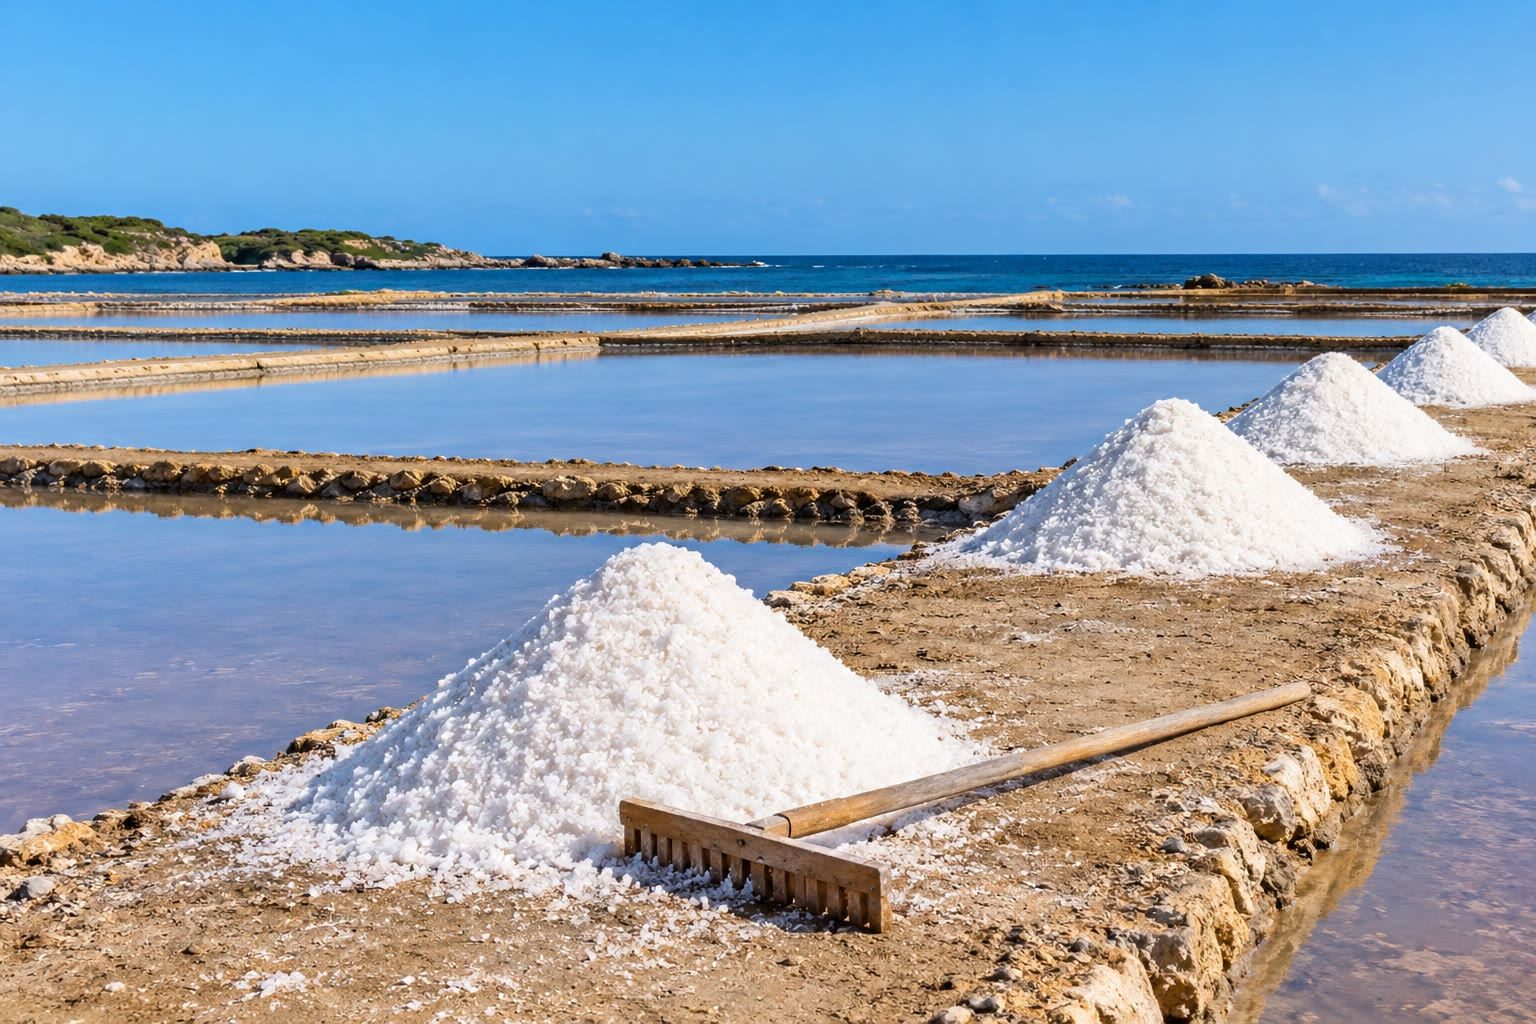
\includegraphics[width=0.62\linewidth]{images/book1/ai/g2-salt-pans.jpg}

{\small أحواض ملح على شاطئ البحر: تجفف الشمس الماء، ويبقى الملح في
أكوام بيضاء.}
\end{omfigure}

\begin{remark}[الذوبان ليس انصهارًا]\label{rem:g2:mixing-and-dissolving:not-melting}
يقول بعض الناس إن السكر «ينصهر» في الشاي. وهذا غير صحيح: الانصهار
هو ما يحدث لمكعب الجليد في الشمس، إذ يصير سائلًا من تلقاء نفسه، دون
حاجة إلى ماء. أما السكر في الشاي فيحتاج إلى الماء، ويبقى السكر فيه
منتشرًا. والكلمة الصحيحة هي \emph{\omterm{def:g2:mixing-and-dissolving:dissolve}{يذوب}}.
\end{remark}

\section{تمارين}

\begin{exercise}[$\star$]\label{exo:g2:mixing-and-dissolving:1}
أي هذه الأجسام الصلبة \omterm{def:g2:mixing-and-dissolving:dissolve}{يذوب} في الماء، وأيها لا \omterm{def:g2:mixing-and-dissolving:dissolve}{يذوب}؟ السكر، والرمل،
والملح، والطباشير، والحصى.
\end{exercise}

\begin{exercise}[$\star$]\label{exo:g2:mixing-and-dissolving:2}
ما \omterm{def:g2:mixing-and-dissolving:dissolve}{المحلول}؟ أعطِ مثالين من هذا الفصل.
\end{exercise}

\begin{exercise}[$\star$]\label{exo:g2:mixing-and-dissolving:3}
هل صحن الموسلي خليط؟ وهل لا تزال ترى كل جزء من أجزائه؟
\end{exercise}

\begin{exercise}[$\star$]\label{exo:g2:mixing-and-dissolving:4}
نحرّك مسحوقًا أبيض في كأس ماء. وبعد بضع دقائق يصير الماء عكرًا
وتتكوّن طبقة بيضاء في القاع. هل ذاب المسحوق؟ علّل اعتمادًا على
\cref{met:g2:mixing-and-dissolving:test}.
\end{exercise}

\begin{exercise}[$\star$]\label{exo:g2:mixing-and-dissolving:5}
كأس من ماء الشراب لونها وردي. هل هي رائقة؟ وهل هي عديمة اللون؟ وهل
هي \omterm{def:g2:mixing-and-dissolving:dissolve}{محلول}؟
\end{exercise}

\begin{exercise}[$\star$]\label{exo:g2:mixing-and-dissolving:6}
بعد التحريك لا يُرى أي سكر في فنجان الشاي. اذكر العلامة التي تدل على
أن السكر لا يزال موجودًا.
\end{exercise}

\begin{exercise}[$\star$]\label{exo:g2:mixing-and-dissolving:7}
في أحواض الملح، ماذا تأخذ الشمس، وماذا يبقى؟
\end{exercise}

\begin{exercise}[$\star$]\label{exo:g2:mixing-and-dissolving:8}
يقول توم: «انصهر السكر في الشاي.» أي كلمة كان عليه أن يستعملها
بدلًا منها، ولماذا؟
\end{exercise}

\begin{exercise}[$\star\star$]\label{exo:g2:mixing-and-dissolving:9}
انظر إلى الشكل الذي فيه الكأسان. كيف تعرف أي الكأسين فيها الرمل، دون
أن تقرأ الكلمات المكتوبة تحتهما؟
\end{exercise}

\begin{exercise}[$\star\star$]\label{exo:g2:mixing-and-dissolving:10}
تجف قطرة من ماء الصنبور على صحن أسود وتترك حلقة بيضاء صغيرة. ماذا
يخبرنا هذا عن ماء الصنبور؟
\end{exercise}

\begin{exercise}[$\star\star$]\label{exo:g2:mixing-and-dissolving:11}
في المختبر، لدى معلمة كأسان فيهما سائل رائق عديم اللون: في إحداهما ماء
نقي، وفي الأخرى ماء مالح. ولا يجوز لأحد أن يتذوقهما. كيف تعرف أيهما
هو أيهما؟
\end{exercise}
